\chapter{Monte Carlo Simulation}\label{chapt:MC}

To analyze the data from a large particle physics experiment, the modeling of the events and of the detector
plays an essential role. The processes of $pp$ interaction and particle production are usually too complicated
to be described in every aspect analytically. The same applies to the interactions within the detector volume. However, these 
tasks can be solved with the help of Monte Carlo (MC) simulation programs. These programs can be used to predict
the signal and background processes event yields and to simulate the detector response including efficiency and smearing effects.

In this analysis it is needed to simulate the whole process $pp \rightarrow t\bar{t} \rightarrow \bar{l}\nu bl\bar{\nu}\bar{b}$, 
including the subsequent reaction steps (see Fig. \ref{fig:pp_all}). First the hard scattering has to be
simulated to describe the collision and production of partons. Then parton showering tools have to be applied 
to describe the electromagnetic and QCD radiation of the initial and the final step particles. In the end of the 
process all the radiation finishes with forming the hadrons. There is also a possibility of interaction with the 
proton remnants. This interaction is described with the underlying event process.

\begin{figure}[t]
  \centering
  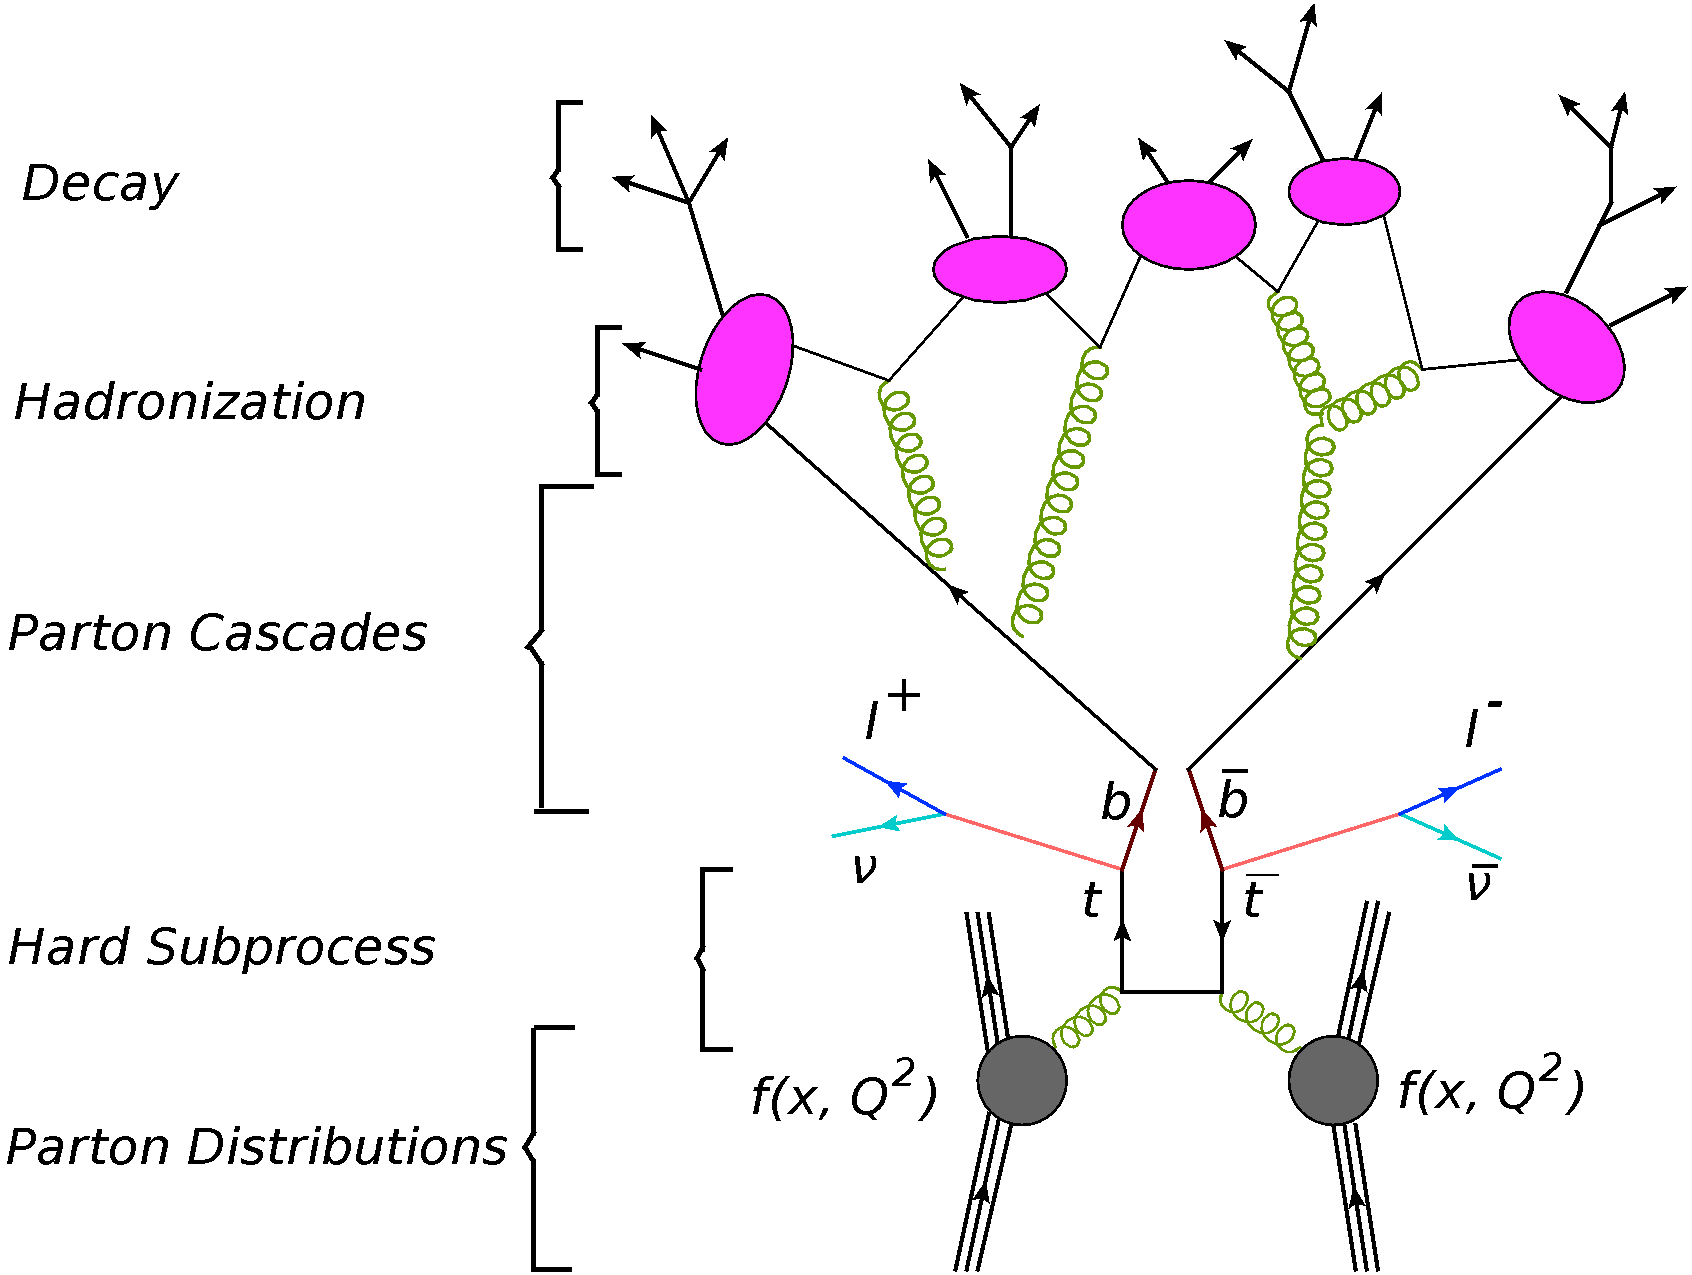
\includegraphics[width=0.8\textwidth]{03_simulation/plots/pp_all_proc.png}
  \caption{$pp$ collision sketch showing all the subprocesses.}
  \label{fig:pp_all}
\end{figure}

There exists a number of general-purpose Monte Carlo (GPMC) generators (HERWIG \cite{Corcella:2000bw}, \PYTHIA6 \cite{Sjostrand:2006za}, 
SHERPA \cite{Gleisberg:2003xi}), which provide a full simulation of high-energy collisions. They consist of several components,
which describe the process on all the interaction scales, starting from the perturbative QCD on the very small distances up to
the QCD-inspired models on the distance scales of hadron formation and decay. 

To finalize the analysis modeling, after simulating the particle production and decay processes, it is necessary 
to ``push" the products of this simulation through a model detector. The model detector simulates the interaction of particles 
with the detector materials and the detector response including noise. Such a detector model can be also used to predict the performance 
of future facilities.

This chapter gives a brief overview of the processes which were simulated for this analysis and tools used for 
the simulation.

\section{Different Monte Carlo Models and Generators}
\subsection{Hard Scattering Models}

The \textit{hard scattering} describes the interaction of partons which emerge out of the proton (in the case of this analysis 
-- two gluons or an quark-antiquark pair) and take part in the production process which is being studied. The initial momenta 
of partons are to be chosen according to the used PDFs (see sec. \ref{ssec:tt_prod}).

The parton interaction is taking place in the high energy regime, so that $\alpha_{s} \ll 1$ (see sec. \ref{sec:strong_int}). 
This allows to perturbativly calculate the process in different orders of $\alpha_{s}$: the higher the order used
for the calculations, the more precise the calculation should be. However, there are many subtleties with calculating 
higher orders, that is why the MC generators are usually limited to LO or NLO calculations.


\subsection{Parton Showering}

The hard scattering models are usually restricted to a fixed order of perturbation theory. This is not sufficient to describe the 
whole picture of the event. That is why special \textit{parton showering} techniques were developed to simulate 
higher order effects. It describes the radiation of the colored objects from initial and final state partons,
following the momentum transfer from the higher interaction scales down to the lowest scales of confinement (hadronization) --
to the order of 1 GeV.

% Parton showering describes two kinds of radiation: \textit{initial state radiation}, or the radiation of colored partons
% before they enter the hard interaction, and the \textit{final state radiation}, or the radiation of inside or at the final
% state of the hard scattering.

\begin{itemize}
 \item \textbf{The final state radiation} is described by sequential splitting of the colored objects with energy decreasing
 after each splitting. This process is repeated until some evolution criterion is reached. Such criteria may be connected
 with the energy fraction of a radiated object or with the opening angle between the parent and emitted colored object.
 
 \item \textbf{The initial state radiation} is produced in the similar way to the final state radiation, but inverting
 the process such that the colored objects out of the shower collapse back to the initial partons out of the protons.
\end{itemize}

If the parton shower is simply added to the hard scattering, the same process can be modeled twice. Some radiation
may be already taken to account in the hard interaction but it is still produced in the parton showering. The problem 
is treated by employing matching mechanisms \cite{Buckley:2011ms}.

\subsection{Hadronization Models}

In context of the MC generators, the \textit{hadronization} is the process by which a set of colored objects (after showering)
is transformed into color-singlet particles, hadrons, which can further decay into other hadrons. This transition is non-perturbative
with the scale $Q_{had}$ (with $\alpha_{s} \sim 1$), which is identical to the shower energy limit. Thus, full QCD calculations
are not possible. The hadronization scale may be defined slightly different in different generators.
% 
% The main difference between the MC hadronization model and fragmentation function description of hadronization in QCD, is that former
% is defined only at the hadronization scale, while the letter is defined at any scale.

There are two models which are the basis for the MC generator hadronization:

\begin{itemize}
 \item \textbf{String model}. The basics for this model were taken from the string model of elementary particle physics \cite{Artru:1974hr}.
 The main feature being exploited is the \textit{linear confinement}, the potential of the color dipole 
 between the color and anticolor is growing linearly with the separation of the color charges up to distances of about a femtometer.
 
 One of the most popular generator string models is the \textit{Lund model}\cite{ANDERSSON1987513}. The linear color potential between the quarks is 
 expressed as $V(r) = \kappa r$, which can be described as a string with tension $\kappa \sim 1\,\text{GeV}/fm \sim 0.2\,\text{GeV}^{2}$. 
 The Coulomb interaction is neglected. The physical picture of this potential is a colored tube between quark
 and antiquark. As the quarks start to separate in space, the string grows and finally breaks via the process of a new quark-antiquark
 pair creation, $q\bar{q} \rightarrow q\bar{q}' + q'\bar{q}$. The illustration of this process is shown in Fig. \ref{fig:Lund}. 
 \begin{figure}[h]
  \centering
  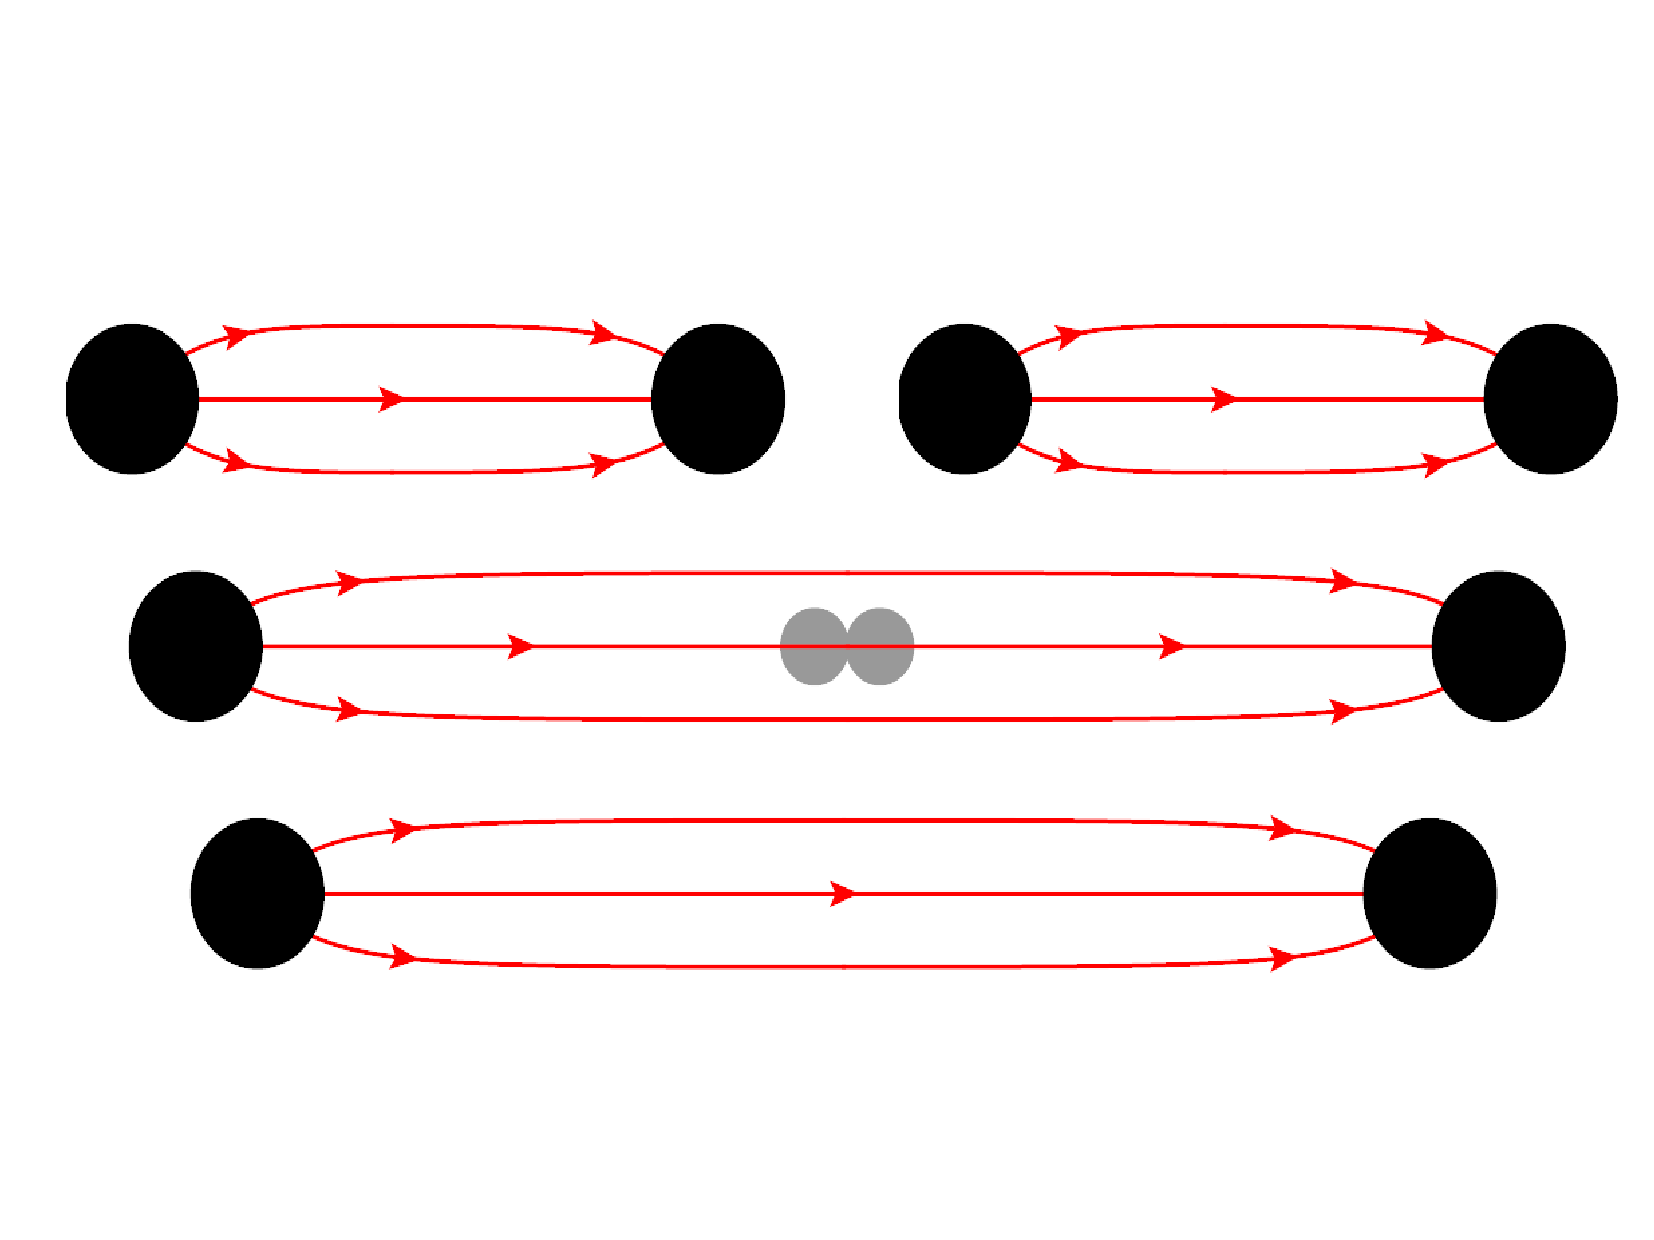
\includegraphics[width=0.8\textwidth]{03_simulation/plots/Lund_hadr.pdf}
  \caption{Illustration of string breaking by quark pair-creation in the string field. Black spots are the quarks and the red
  strips are the field illustration.}
  \label{fig:Lund}
 \end{figure} 
%  The gluons are represented with transverse kinks in the strings. They have to be connected to the field strings from both
%  sides, while quarks have connection only from one side.
%  
 In the mechanism described above, mesons are produced if after the string breaking states with two quarks are formed. 
 Baryons can be also produced, but in the process where the string breaking produces a pair of diquarks.
 The hadronization stops after reaching the point when there is not enough energy to create another hadron.
 
 \item \textbf{Cluster model}. This hadronization model is based on the \textit{preconfinement} \cite{Amati:1979fg}, or the
 observation that the color-singlet parton subsystems, called \textit{clusters}, occur with universal mass distribution
 depending only on the scale $Q_{0}$ at which they were formed, and not on the starting scale of the showering.
 The other key idea of the model is that the gluons are forced to split into a quark-antiquark pair at the end of the parton shower.
 The clusters formed by the gluon splitting are then forced to decay into on-shell hadrons. The cluster hadronization in comparison
 to string hadronization is represented in Fig. \ref{fig:clustHad}.
 
 \begin{figure}[h]
  \centering
  \begin{subfigure}
   \centering
   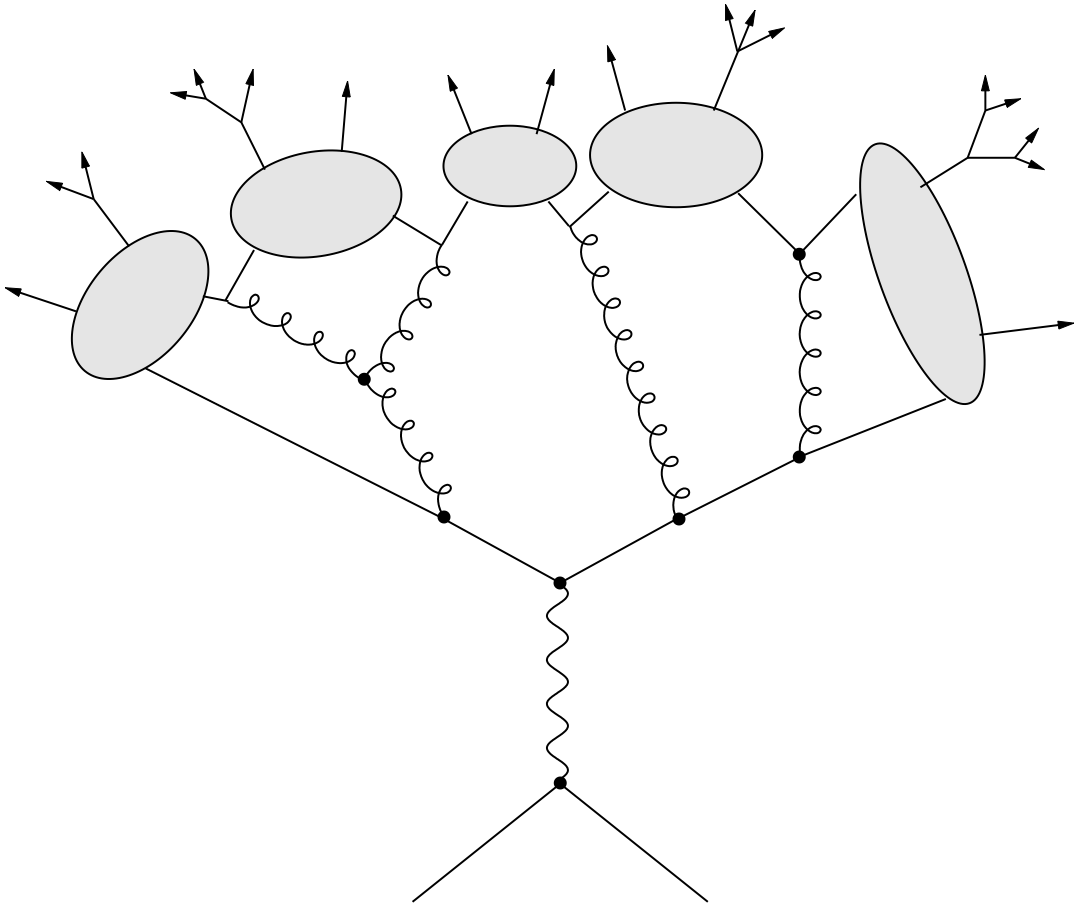
\includegraphics[width=0.49\textwidth]{03_simulation/plots/Figures_MonteCarlo_clustr_had.png}
  \end{subfigure}
  \begin{subfigure}
   \centering
   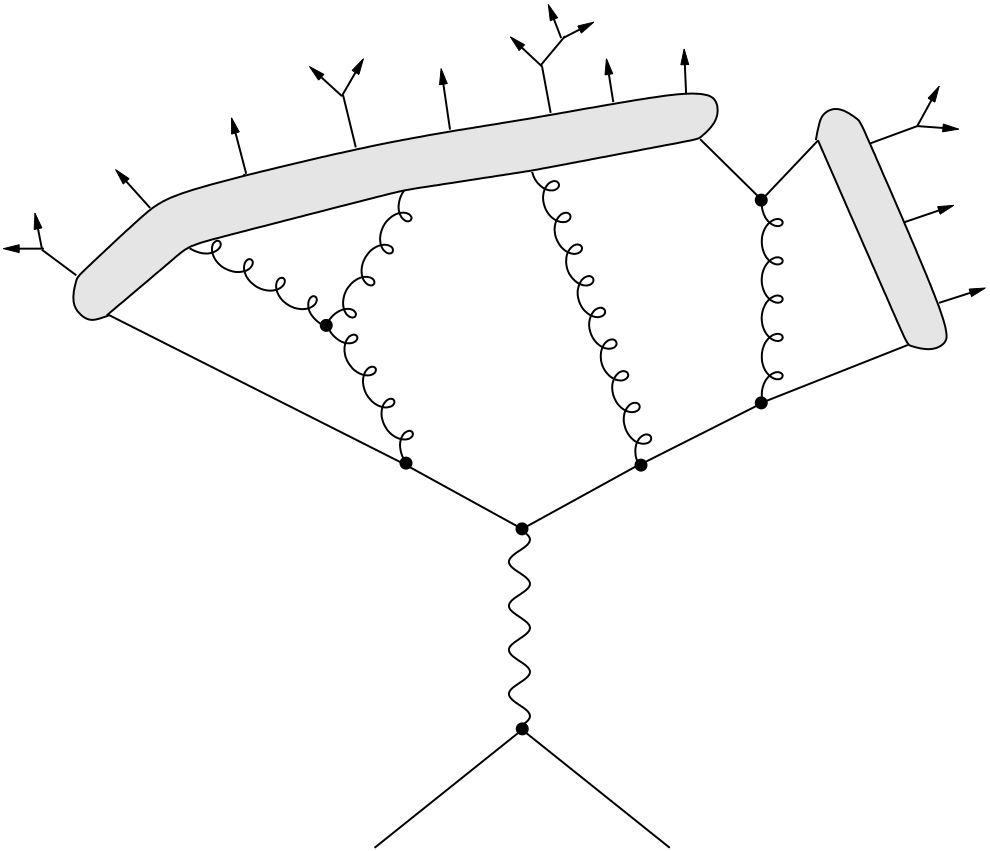
\includegraphics[width=0.49\textwidth]{03_simulation/plots/Figures_MonteCarlo_string_had.png}
  \end{subfigure}
  \caption{Illustration of cluster (left) and string (right) hadronization model. The figure is taken from \cite{Webber:1999ui}.}
  \label{fig:clustHad}
 \end{figure} 
 
\end{itemize}

\subsection{Hadron Decay}

The hadrons formed after hadronization, are so-called primary hadrons. They can be unstable and they decay into secondary hadrons
until the set of stable particles\footnote{A typical definition of stable particles in hadron colliders is that their
lifetime, $c\tau$, is greater than 10 mm. This includes the weakly decaying strange baryons.} is formed.

One would expect, that all the needed information for the decay would be present in the Particle Data Group (PDG) listings \cite{PDG-2012}.
However, this information is often not complete and requires multiple choices to be made. The more hadrons are included into the simulation,
the more choices one has to make.

The individual properties of each generator are:

\begin{itemize}
 \item which hadrons to include into simulation;
 \item which decay modes to allow;
\end{itemize}

In general, the simulation of hadron decays is based on a combination of experimentally measured properties and theoretical assumptions, which
might also differ from generator to generator.

\subsection{Underlying Event}

The \textit{underlying event} (UE), is, in terms of the MC generators, the activity beyond the hard process, like multiple parton-parton interactions
(MPI) between the beam particles and the hadronization of beam-beam remnants (BBR) \cite{Khachatryan:2015pea}. The BBR include hadrons from the partons 
which do not exchange any appreciable $p_{T}$ in the collision. The MPI may sometimes give a rise to two or more back-to-back jets (if there were more 
hard parton-parton interactions in one proton-proton collision). This case is, however, very rare. The main impact is coming from the soft MPI. They may 
affect, for example, the missing $E_{T}$ distribution or increase the activity in the forward direction (break-up of the beam remnants).

% The basic Monte Carlo model for the UE is given in \cite{PhysRevD.36.2019}. There are some basic assumptions involved in
% this model, like, for example, the interactions can't use more momentum than it is available in the parent hadron (proton in case of this analysis).

The UE models are usually tuned to the experimental conditions and on experimental data. The model derived on the CMS data collected at $\sqrt{s} = 0.9\, TeV$
and $\sqrt{s} = 8\,TeV$ is called the $Z2*$ tune \cite{Chatrchyan:2011id}.


\subsection{Monte Carlo Generators}

After describing the main principles behind the MC simulation of the events for the experiments in the field of elementary particle
physics, the list of the generators used for this analysis will be given in the following:

\subsubsection{$\PYTHIA$ 6}

\PYTHIA \cite{Sjostrand:2006za} is a general-purpose event generator. It models $pp$, $\gamma p$ and $e^{+}e^{-}$ collisions. \PYTHIA includes more than 200 hardcoded
hard subprocesses, which include the Standard Model reactions but also some exotic beyond Standard Model processes \cite{Buckley:2011ms}.
%
The matrix elements of the hard parton scattering are calculated in \PYTHIA in LO QCD accuracy.
%
For the parton showering, the parton emissions are ordered by the transverse momentum of the radiating parton, $Q^{2} = p_{T}(part.)$.
%
For the hadronization, the Lund string model is used.
%
Particle decays are included in $\PYTHIA$, using specific decay tables containing all relevant decay branching ratios.
%
The $Z2*$ tune for the UE simulation is conventionally (for the CMS experiment) used in \PYTHIA for the UE simulation for this analysis.

\subsubsection{$\HERWIG$ 6}

\HERWIG \cite{Corcella:2000bw} is a general-purpose LO matrix element plus parton shower generator like \PYTHIA. It can model hadron-hadron, 
lepton-lepton and hadron-lepton collisions.
%
\HERWIG is able to produce a fairly large variety of Standard Model QCD, electroweak processes and elementary subprocesses beyond the standard model.
%
The parton showering is ordered by the scale $Q^{2} \sim 1 - \cos\theta$, where $\theta$ is the angle between the parent and emitted partons.
%
The cluster model is used for the hadronization in \HERWIG.
%
The model for the UE used here by \HERWIG was originally derived by ATLAS and is called AUET2 \cite{ATL-PHYS-PUB-2011-009}.

\subsubsection{MadGraph}

\MG\cite{Alwall:2011uj} is another general-purpose generator. It can be used to generate the hadron-hadron $pp$ and $p\bar{p}$, as well as the other types of collisions.
It gives the LO matrix elements for hard processes with up to 8 particles in the final state. 

\MG is a pure matrix element generator. It doesn't include hadronization and provides only leptons, quarks and gluons as outgoing hard particles. 
The outcome is afterwards interfaced to some general-purpose generator to generate further steps (parton showering, hadronization). 
% The combination $\MG+\PYTHIA$ 
% provides better results compared to \PYTHIA only, as the \MG hard interaction is more specifically tuned than \PYTHIA for the needs of hadron-hadron collisions. 

The problem of double counting of objects in showering, while interfacing \MG to the general-purpose generator, is solved with the help of the 
MLM scheme \cite{Mrenna:2003if}. In this scheme the showered partons are generated in a restricted phase space with a minimal cone separation
between each other. These partons are clustered into jets using the cone algorithms. If the original parton is included in more than one jet,
the event is rejected.

For this analysis the PDF CTEQ6L1 set \cite{Pumplin:2002vw} is used in \MG to describe the proton structure.

\subsubsection{Powheg}

The \Powheg (Positive Weight Hardest Emission Generator) event generator \cite{Frixione:2007vw} provides the modeling of the hard interaction 
with NLO accuracy. The \Powheg method doesn't have parton showering included. Thus, it has to be also interfaced with \PYTHIA or
\HERWIG for a full event description. For the description of proton structure, the CT10 \cite{Lai:2010vv} PDFs are used.

\subsubsection{MC@NLO}

The \MCNLO \cite{Frixione:2002ik} is also an event generator which generates the hard emission with NLO precision. For the showering
it has to be interfaced with general-purpose generators, as it is also done for \Powheg. 

\MCNLO is designed for hadron collisions with production of top quark pairs, Higgs boson, vector boson (single or in pairs), single top,
lepton pairs and associated $H+W/Z$.

The \MCNLO generator provides some events with negative weights. However, the fraction of these events is very small \cite{Frixione:2002ik}.

The CTEQ6M \cite{Pumplin:2002vw} PDF sets were exploited in \MCNLO for this analysis.


\section{Detector simulation}

After the bare event with all the particles is simulated, it can be ``pushed through" a detector simulation. That means that all of the particles 
will interact with the materials and electromagnetic fields of the model of a real detector. This allows the estimation of 
detector efficiencies and smearing of observables such as particles energies, prediction of the performance and comparison of the theoretical 
models encoded in the event generators to
the experimental measurements. The simulation of the detector is performed by means of the Geant simulation toolkit.

\subsubsection{Geant 4}

Geant4 (GEometry ANd Tracking) \cite{Agostinelli:2002hh} is a toolkit designed for an accurate simulation of the passage of particles through matter.
The tool includes all the aspects of the simulation, like the geometry of the system, the materials involved, fundamental particles of interest,
tracking of particles through materials and electromagnetic fields, the physics processes governing the particle interactions, the response of
sensitive detector components, the storage of events and tracks, the vizualization of detector and particle trajectories and the analysis of
the data on different levels of details.

Geant can handle the particle interactions on a very wide energy scale. It also includes a large amount of known particle interaction models.

For the needs of the CMS experiment Geant4 is used for the detector simulation. An example of the display of a fully simulated CMS $t\bar{t}$ event
in the $e\mu$ decay channel is shown in Fig. \ref{fig:Evt_display}.

 \begin{sidewaysfigure}[p]
  \centering
  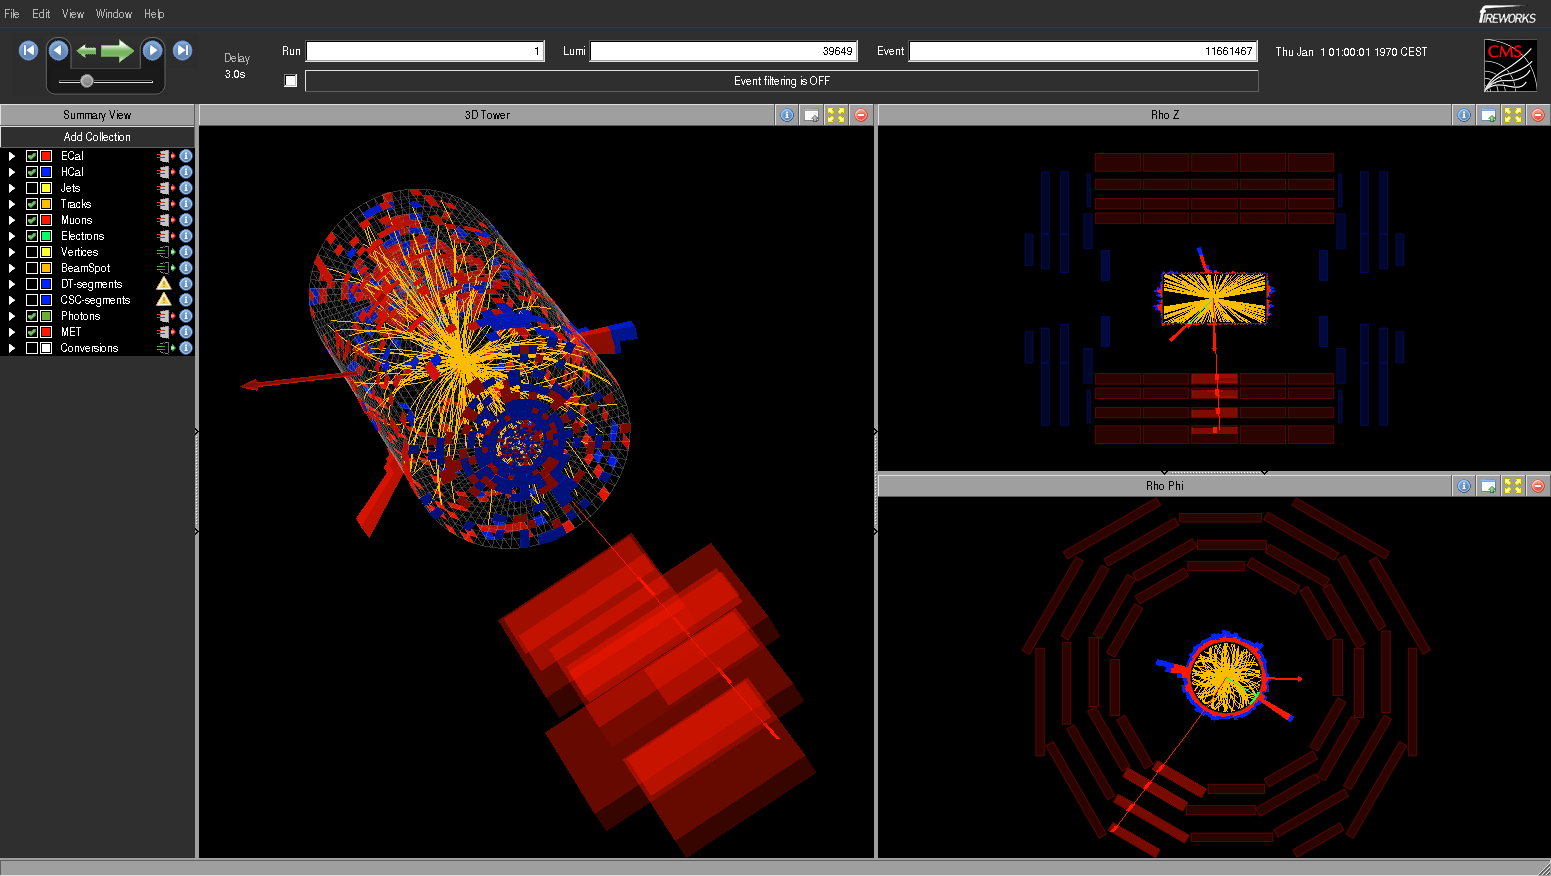
\includegraphics[width=1.0\textwidth]{03_simulation/plots/eventDisplay-39649-11661467.png}
  \caption{Display of a simulated $t\bar{t}$ event in the CMS detector model, produced with the CMS event display.}
  \label{fig:Evt_display}
 \end{sidewaysfigure}